% =============================================================================
%                       ESTADO DEL ARTE Y MARCO TEÓRICO
% =============================================================================

\cleardoublepage

\chapter{Estado del Arte y Marco Teórico}
\label{estado-del-arte-marco-teorico}

Este capítulo recorre las bases teóricas y empíricas sobre las que se asienta el presente Trabajo de Fin de Máster. Se estructura en tres bloques: (i) los \emph{fundamentos sismológicos clásicos}, que delimitan qué se entiende por terremoto, por \textit{mainshock} y por sismicidad observable (Sección \ref{fundamentos-sismologia}); (ii) los \emph{métodos estadísticos clásicos de pronóstico sísmico}, con la familia ETAS como referente (Sección \ref{metodos-estadisticos-clasicos}); y (iii) los \emph{métodos basados en aprendizaje profundo}, agrupados por tipo de arquitectura y problema sismológico abordado (Secciones \ref{dl-fundamentos}--\ref{dl-incertidumbre}). El capítulo cierra con una revisión de los \emph{trabajos relacionados} más cercanos al planteamiento integrado de este TFM (Sección \ref{trabajos-relacionados}).

\section{Fundamentos sismológicos clásicos}
\label{fundamentos-sismologia}

\subsection{Caracterización de un terremoto}
\label{caracterizacion-terremoto}

Un terremoto es un evento geológico caracterizado por la liberación brusca de energía elástica acumulada en la corteza y el manto superior de la Tierra debida a la fricción en las fallas \citep{stein2003introduction}. Su descripción cuantitativa se apoya en cinco parámetros fundamentales: \emph{tiempo de origen} $t_0$, \emph{hipocentro} (latitud, longitud, profundidad) y \emph{magnitud} $M$. La magnitud, en el sentido moderno (\textit{moment magnitude}, $M_w$), se relaciona con el momento sísmico escalar $M_0$ --expresado en N$\cdot$m (unidades del Sistema Internacional)-- mediante la fórmula recogida en el \emph{New Manual of Seismological Observatory Practice} \citep{bormann2012nmsop, bormann2011mw}:

\begin{equation}
  M_w = \tfrac{2}{3}\left( \log_{10}(M_0) - 9.1\right)
  \label{eq:Mw}
\end{equation}

La constante $9.1$ resulta de convertir la formulación original de Kanamori \citep{hanks1979moment}, planteada en CGS con $M_0$ en dyn$\cdot$cm, al SI con $M_0$ en N$\cdot$m (factor de conversión $1$\,N$\cdot$m $= 10^{7}$\,dyn$\cdot$cm). La energía sísmica radiada $E$ se estima mediante la relación de Gutenberg--Richter \citep{gutenberg1956energy}, equivalente a la formulación de \citet{kanamori1977energy} y que se expresa en su forma SI como \citep{bormann2012nmsop, bormann2011mw}:

\begin{equation}
  \log_{10} E\,[\mathrm{J}] = 1.5\, M + 4.8
  \label{eq:kanamori}
\end{equation}

La constante $+4.8$ resulta de convertir la expresión original $\log_{10} E\,[\mathrm{erg}] = 1.5\,M + 11.8$ \citep{gutenberg1956energy} al SI ($1$\,J $= 10^{7}$\,erg). La ecuación (\ref{eq:kanamori}) implica que un incremento de una unidad de magnitud corresponde a un factor $\sim 31.6\times$ en energía liberada; este escalado motivará el uso de $\log_{10}(1+E)$ como \textit{feature} en los modelos descritos en el capítulo \ref{desarrollo-del-proyecto-y-resultados}.

\subsection{Las ondas P y S}
\label{ondas-p-s}

Las ondas sísmicas se clasifican en ondas \emph{de cuerpo} (P y S) y \emph{superficiales} \citep{shearer2009introduction, stein2003introduction}. Las ondas P (\textit{primary}) son longitudinales, viajan a velocidades aproximadas de $5$--$8$\,km/s en la corteza y son las primeras en alcanzar la estación receptora. Las ondas S (\textit{secondary}) son transversales, más lentas ($3$--$5$\,km/s) y típicamente más destructivas. La \emph{detección} automática de un evento sísmico se reduce, en términos prácticos, a identificar las llegadas de estas dos fases sobre los sismogramas continuos. La diferencia $t_S - t_P$ es proporcional a la distancia epicentro-estación, y la triangulación con varias estaciones permite localizar el evento.

\begin{figure}[ht!]
  \centering
  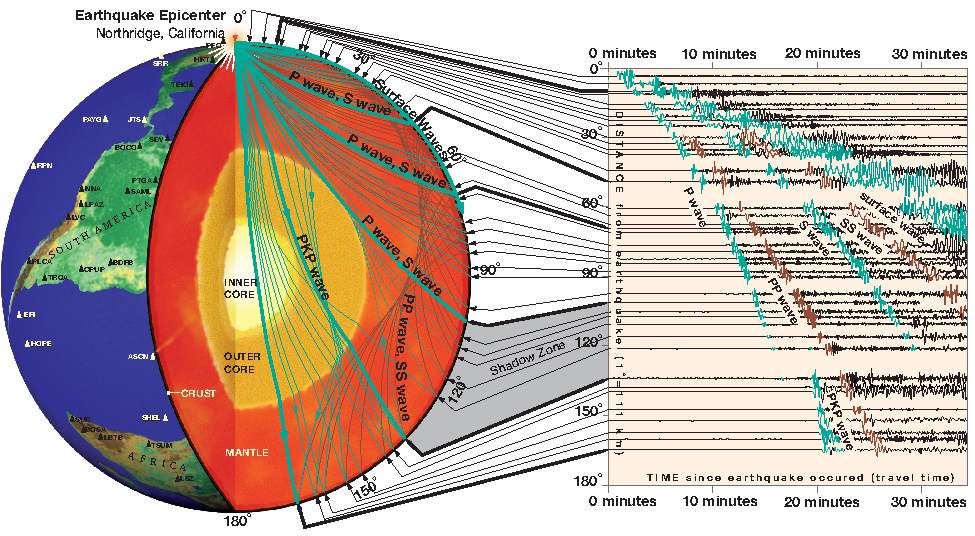
\includegraphics[width=0.8\textwidth]{figuras/ondas_p_s}
  \caption[Trayectorias y tiempos de viaje de las ondas P y S a través del interior de la Tierra \citep{iris2010seismology}]{\textbf{Trayectorias y tiempos de viaje de las ondas sísmicas a través del interior de la Tierra para el terremoto de Northridge (California, 17 de enero de 1994, $M_w$ 6.9).} Se muestran los caminos seguidos por las ondas P, S, PP, SS, PKP y superficiales al atravesar las diferentes capas terrestres; se aprecia la \textit{shadow zone} entre los $100^{\circ}$ y los $140^{\circ}$ donde las ondas P directas dejan de llegar al desviarse al atravesar el núcleo externo. También aparecen los sismogramas registrados en estaciones repartidas por el planeta, con la separación temporal creciente entre la llegada de las ondas P, S y superficiales en función de la distancia angular al epicentro \citep{iris2010seismology}.}
  \label{fig:ondas-ps}
\end{figure}

Estas dos tareas --detección de eventos y \textit{picking} preciso de las llegadas P/S-- han sido tradicionalmente abordadas por algoritmos heurísticos como STA/LTA (\textit{short-term average over long-term average}) y \textit{template matching} por correlación cruzada. Su limitación principal es la cantidad de falsos positivos en presencia de ruido o eventos solapados. El aprendizaje profundo ha desplazado en pocos años este campo mediante arquitecturas como PhaseNet \citep{zhu2018phasenet} y EQTransformer \citep{mousavi2020eqtransformer}, que se describen en la Sección \ref{dl-sismologia}.

\subsection{Ley de Gutenberg--Richter y \textit{b-value}}
\label{ley-gr}

La distribución de magnitudes en un catálogo sísmico sigue empíricamente una ley exponencial conocida como \emph{ley de Gutenberg--Richter} \citep{gutenberg1944frequency}, la cual relaciona la frecuencia de ocurrencia con la magnitud del terremoto:

\begin{equation}
  \log_{10} N(M) = a - b\, M,
  \label{eq:gr}
\end{equation}

donde $N(M)$ es el número de eventos con magnitud mayor o igual que $M$, $a$ caracteriza la productividad sísmica regional y $b$ es la pendiente, denominada \emph{b-value}, representa la relación entre sismicidad de pequeña y gran magnitud. Para regiones tectónicamente activas $b$ suele oscilar en torno a $1.0$ \citep{frohlich1993bvalues}, aunque variaciones temporales y espaciales del $b$-value tienen significado físico: $b$ es inversamente proporcional al estado de \emph{stress} acumulado en la corteza, de modo que decrementos transitorios del $b$-value preceden a algunos terremotos grandes \citep{schorlemmer2005bvalue}. Esta es precisamente una de las hipótesis precursoras que se evalúan en el capítulo \ref{desarrollo-del-proyecto-y-resultados}.

El estimador máximo verosímil del $b$-value es debido a \citet{aki1965bvalue}:
\begin{equation}
  \hat{b} = \frac{\log_{10}(e)}{\bar{M} - (M_c - \Delta M/2)},
  \label{eq:b-aki}
\end{equation}
con $\bar{M}$ la magnitud media de los eventos con $M \geq M_c$, $M_c$ la \emph{magnitud de completitud} del catálogo y $\Delta M$ el paso de discretización (típicamente $0.1$).

La Figura~\ref{fig:gr-cal-alaska} ilustra empíricamente la ley de Gutenberg--Richter sobre los catálogos USGS de California y Alaska (2010--2024). El ajuste sobre California (23\,322 eventos $M\geq 2.5$) arroja $b = 0.90$, valor que cae entre los regímenes de alto $\mathit{stress}$ ($b=0.8$ \citep{schorlemmer2005bvalue}) y el canónico global ($b=1.0$ \citep{frohlich1993bvalues}), coherente con un régimen tectónico transformante. Alaska (71\,026 eventos), por su parte, presenta $b = 0.74$, sensiblemente más bajo, lo que es consistente con un régimen de subducción donde se acumula proporcionalmente más sismicidad grande respecto a la pequeña \citep{wiemer2002mapping, frohlich1993bvalues}. La desviación de los datos respecto a la recta para magnitudes $M\gtrsim 6.5$ corresponde a los pocos eventos grandes registrados en el periodo y refleja la incertidumbre estadística esperada en la cola de la distribución.

\begin{figure}[ht!]
  \centering
  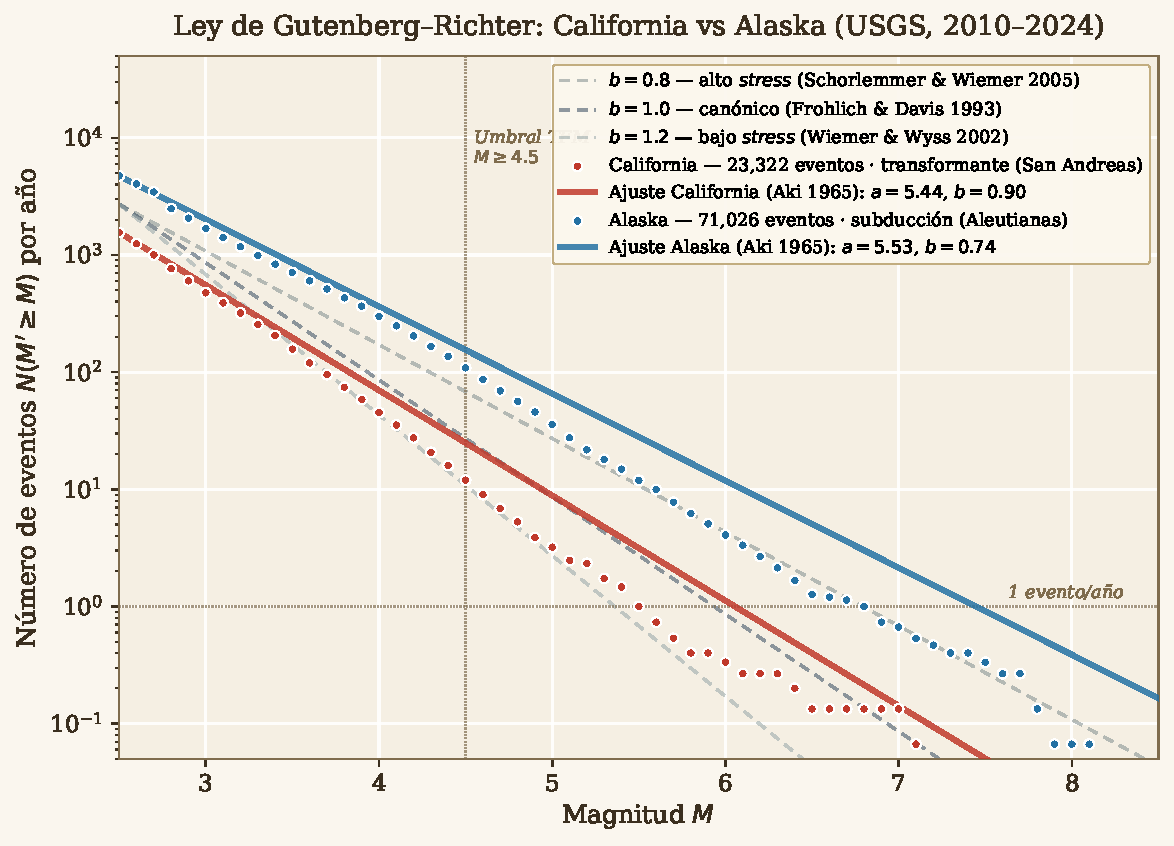
\includegraphics[width=0.95\textwidth]{figuras/figura_gr_california}
  \caption[Ley de Gutenberg--Richter empírica para California y Alaska (USGS 2010--2024)]{\textbf{Validación empírica de la ley de Gutenberg--Richter sobre los catálogos USGS de California y Alaska (2010--2024).} Los puntos representan la frecuencia acumulada anual de eventos por encima de cada magnitud; las líneas continuas son los ajustes máximo verosímiles obtenidos mediante el estimador de \citet{aki1965bvalue}, corregido por binning. Las líneas discontinuas grises muestran tres curvas teóricas de referencia con $b\in\{0.8, 1.0, 1.2\}$ correspondientes a distintos regímenes documentados en la literatura: alto $\mathit{stress}$ \citep{schorlemmer2005bvalue}, canónico global \citep{frohlich1993bvalues} y bajo $\mathit{stress}$ o volcánico \citep{wiemer2002mapping}. California (rojo) presenta $b = 0.90$, coherente con un régimen transformante (falla de San Andreas); Alaska (azul) presenta $b = 0.74$, valor más bajo característico de zonas de subducción (arco de las Aleutianas). Las líneas guía indican el umbral de pronóstico del TFM ($M\geq 4.5$, vertical) y la tasa de un evento al año (horizontal).}
  \label{fig:gr-cal-alaska}
\end{figure}

\subsection{Magnitud de completitud \texorpdfstring{$M_c$}{Mc}}
\label{mc}

La magnitud de completitud $M_c$ es el mínimo valor de $M$ a partir del cual el catálogo se considera estadísticamente completo (no faltan eventos por debajo del umbral de detección de la red de estaciones). Su determinación es un paso preprocesado esencial: \textit{features} agregadas calculadas con $M < M_c$ contaminarían la señal con ruido de selección, y un $M_c$ mal estimado sesga directamente el $b$-value de la ecuación (\ref{eq:b-aki}). Los métodos más utilizados en la literatura son:

\begin{itemize}
  \item \textbf{\textit{Maximum curvature} (MAXC).} Define $M_c$ como el punto de máxima curvatura de la distribución frecuencia--magnitud, equivalente al pico del histograma no acumulado de magnitudes \citep{wiemer2000mc}. Es rápido y fiable pero tiende a \emph{subestimar} $M_c$ en distribuciones suavemente curvadas.
  \item \textbf{\textit{Best combination} (BC).} Variante de MAXC con un intervalo de confianza del 95\,\%, lo que reduce el sesgo a costa de mayor coste computacional \citep{wiemer2000mc}.
  \item \textbf{\textit{Goodness-of-fit test} (GFT) y \textit{b-value stability}.} Métodos clásicos basados en la bondad de ajuste de la recta de G--R por encima de cada candidato a $M_c$ \citep{mignan2012mc}.
  \item \textbf{\textit{Entire-magnitude-range method} (EMR).} El método más robusto actualmente disponible: ajusta simultáneamente un modelo de ley de potencia para la parte completa ($M \geq M_c$) y una función de detección probabilística para la parte incompleta ($M < M_c$), maximizando la verosimilitud conjunta \citep{woessner2005assessing}.
\end{itemize}

Para las redes modernas SCSN/NCSN (California) y AEC (Alaska), la literatura sitúa $M_c \approx 2.0$--$2.5$ a partir del año 2000 \citep{wiemer2000mc}. En este trabajo se adopta $M_c = 2.5$ como umbral conservador, lo que asegura completitud incluso en periodos puntuales de menor cobertura de la red.

\subsection{Ley de Omori--Utsu y réplicas}
\label{omori}

Inmediatamente después de un terremoto grande (denominado \emph{mainshock}), se observa una secuencia de eventos menores --las \emph{réplicas} o \textit{aftershocks}-- cuya tasa de ocurrencia decae con el tiempo según la ley de \citet{omori1894aftershocks}, modificada posteriormente por \citet{utsu1961statistical}:
\begin{equation}
  n(t) = \frac{K}{(t + c)^p},
  \label{eq:omori}
\end{equation}
donde $K$, $c$ y $p$ son parámetros ajustables, siendo $p$ el que describe la tasa de decaimiento. Para California, $p$ se sitúa típicamente entre $0.9$ y $1.3$. La existencia de réplicas tiene una consecuencia metodológica crítica para los modelos de pronóstico: si un catálogo no se \emph{declusteriza}, los eventos no son independientes y cualquier modelo aprenderá a predecir trivialmente la continuación de una secuencia de réplicas, no patrones precursores reales \citep{vanstiphout2012declustering}.

\subsection{\textit{Declustering}: el algoritmo de Gardner--Knopoff}
\label{declustering}

El algoritmo de \citet{gardner1974poissonian} es la técnica de \textit{declustering} más utilizada históricamente. Para cada evento candidato a \textit{mainshock}, define una ventana espacio-temporal alrededor en la que cualquier evento de menor magnitud se considera réplica o \textit{foreshock} dependiente. Las ventanas de Gardner–Knopoff originalmente se publicaron como tabla; \citet{vanstiphout2012declustering} dan la versión continua que se usará en este trabajo:
\begin{align}
  L(M) & = 10^{0.1238\, M + 0.983}\,\,\mathrm{km} \label{eq:gk-L}                   \\
  T(M) & = 10^{0.5409\, M - 0.547}\,\,\text{días}, \quad M \geq 6.5 \label{eq:gk-T}
\end{align}
con una expresión alternativa para $M < 6.5$. Tras el filtrado se obtiene un sub-catálogo de \emph{mainshocks independientes} sobre el que se define el \emph{target} del problema de pronóstico. \citet{reasenberg1985declustering} propuso una variante posterior basada en una ventana modificada de Omori; ambas se consideran válidas en la literatura. La elección de G-K en este trabajo se justifica por su simplicidad, su naturaleza determinista (mismo catálogo entrada $\Rightarrow$ mismo catálogo salida, sin parámetros estocásticos) y su uso extendido como referencia comparativa.

\subsection{Catálogos sísmicos: USGS, SCSN, AEC y catalogos relocados}
\label{catalogos}

El \gls{usgs} mantiene un catálogo sísmico global accesible vía el web service FDSN, que agrega contribuciones de las redes regionales SCSN, NCSN, AEC y otras. Para estudios de más alta precisión existen catálogos relocados mediante métodos de diferencia doble (\textit{double-difference}): el de \citet{hauksson2012relocated} cubre el sur de California desde 1981, y el de \citet{waldhauser2008doubledifference} el norte. Estos catálogos relocados reducen el error de localización por un factor $\sim 10\times$ a costa de cobertura geográfica más restringida; en este TFM se utiliza el catálogo USGS bruto como fuente principal por homogeneidad regional, dejando los relocados como plan B para futuros trabajos.

\section{Métodos estadísticos clásicos de pronóstico sísmico}
\label{metodos-estadisticos-clasicos}

\subsection{De la predicción determinista al pronóstico probabilístico}
\label{prediccion-vs-pronostico}

Desde la década de los 70 hasta los años 90, sucesivos intentos de predicción sísmica determinista (lugar + tiempo + magnitud) resultaron en notorios fracasos, hasta el punto de que \citet{geller1997unpredictable} sintetizó en \textit{Science} la postura mayoritaria de la comunidad: ``los terremotos no pueden predecirse'', en el sentido del determinismo clásico. \citet{jordan2011oef} formalizaron la transición al \emph{pronóstico probabilístico}: en lugar de afirmar que un evento ocurrirá, se estima la probabilidad condicional $P(M \geq M^* \mid \text{\emph{historia}}, \text{\emph{ventana}}, \text{\emph{región}})$. Esto se ha materializado en sistemas operativos como \emph{Operational Earthquake Forecasting} en Italia \citep{marzocchi2014oef} y como el modelo UCERF3 en California \citep{field2014ucerf3, field2017ucerf3etas}. Ambos sistemas se articulan en torno a un mismo motor estadístico, el modelo \emph{Epidemic-Type Aftershock Sequence} (ETAS), que constituye la pieza central de la sismología probabilística clásica.

\subsection{El modelo UCERF3 y \textit{ShakeMap}}
\label{ucerf-shakemap}

El \emph{Uniform California Earthquake Rupture Forecast version 3} \citep{field2014ucerf3} integra geometría de fallas, tasas de deslizamiento geológicas, parámetros ETAS y modelos de propagación para producir mapas de peligrosidad probabilística a 30 días, 1 año, 30 años y 100 años. Su variante UCERF3-ETAS \citep{field2017ucerf3etas} añade la dimensión temporal corta. La Figura~\ref{fig:ucerf3-map} muestra el mapa resultante de UCERF3 para California, donde el color de cada segmento de falla codifica la probabilidad de participación en una ruptura sísmica de gran magnitud. Por su parte, \emph{ShakeMap} \citep{wald1999shakemap} es la herramienta operacional de generación de mapas de intensidad inmediatamente después de un evento. Estos sistemas constituyen el \textit{ground truth} operacional contra el que cualquier modelo de aprendizaje profundo aspira a competir o complementar.

\begin{figure}[ht!]
  \centering
  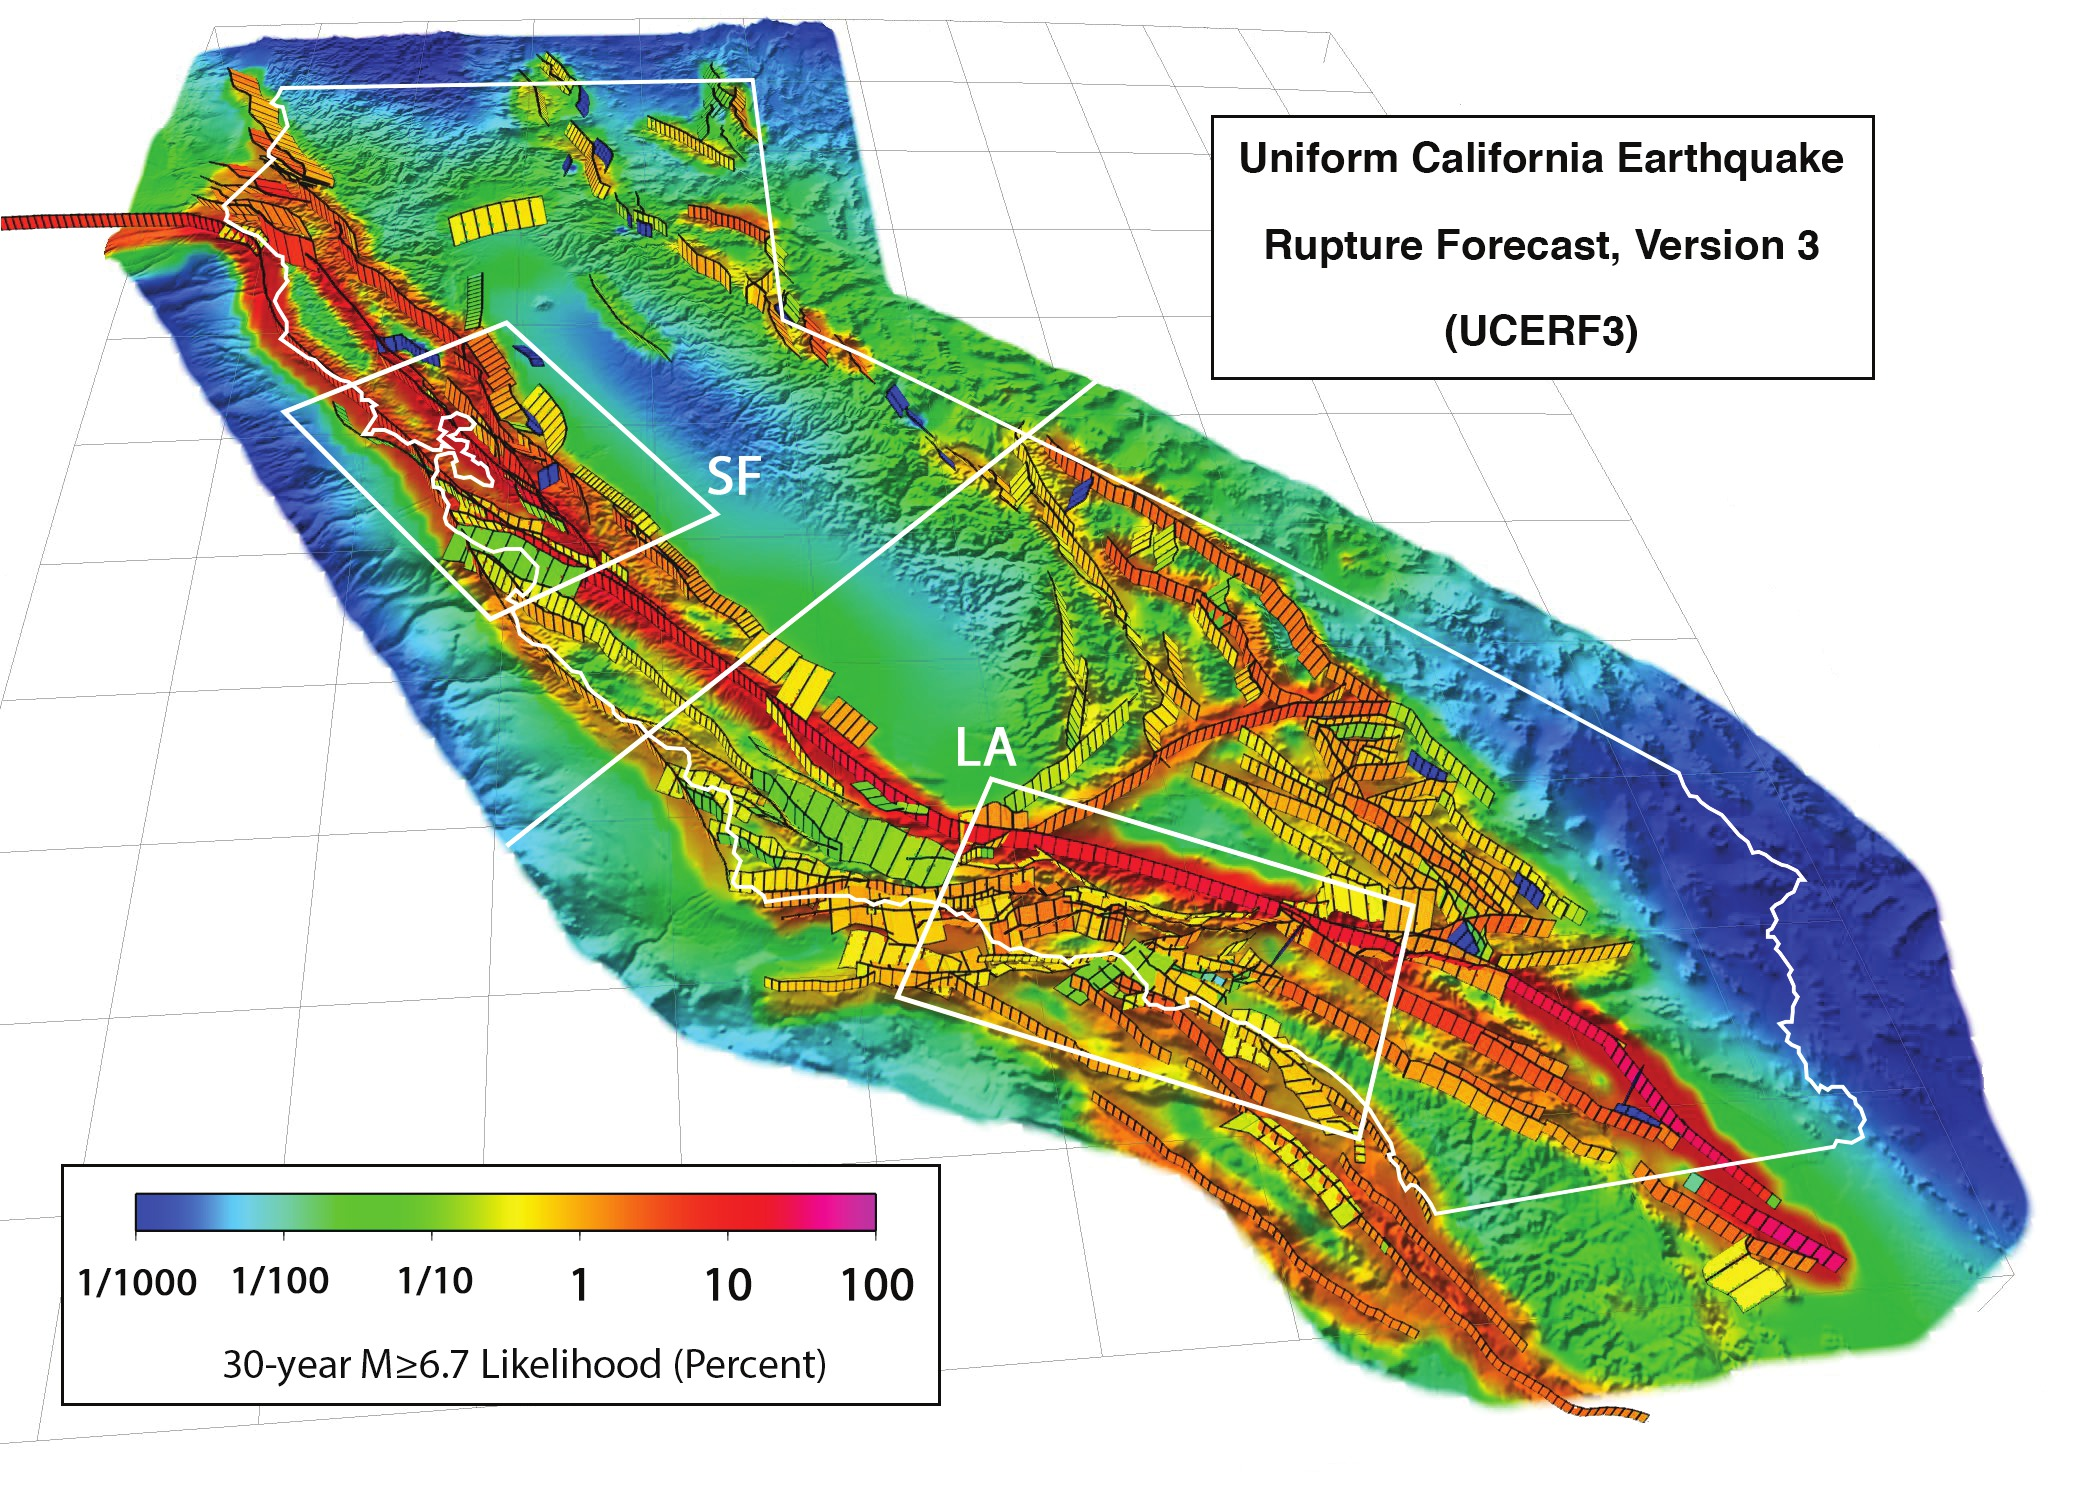
\includegraphics[width=0.85\textwidth]{figuras/figura_UCERF3.png}
  \caption[Mapa UCERF3 de probabilidad de terremoto $M\geq 6.7$ a 30 años en California \citep{wikipediaucerf3, field2015ucerf3factsheet}]{\textbf{Mapa UCERF3 de probabilidad de ocurrencia de un terremoto de $M\geq 6.7$ en los próximos 30 años en California.} El color de cada segmento de falla indica la probabilidad con la que esa sección participará en una ruptura sísmica de dicha magnitud; la falla de San Andrés y la de Hayward concentran las probabilidades más elevadas. El modelo integra geometría de fallas, tasas de deslizamiento geológicas y parámetros ETAS \citep{field2015ucerf3factsheet}. Imagen tomada del artículo divulgativo de Wikipedia sobre UCERF3 \citep{wikipediaucerf3}, prácticamente idéntica a la publicada en el \emph{fact sheet} oficial del USGS \citep{field2015ucerf3factsheet}.}
  \label{fig:ucerf3-map}
\end{figure}

\subsection{La familia ETAS}
\label{etas}

El \emph{Epidemic-Type Aftershock Sequence} de \citet{ogata1988etas, ogata1998spacetime} modela la sismicidad como un proceso de puntos auto-excitante: cada evento incrementa transitoriamente la tasa de ocurrencia en su entorno, con la tasa total $\lambda(t, x, y)$ formulada como
\begin{equation}
  \lambda(t,x,y) = \mu(x,y) + \sum_{i: t_i < t} \frac{K_0\, e^{\alpha(M_i - M_c)}}{(t - t_i + c)^p}\, f(x - x_i, y - y_i; M_i)
  \label{eq:etas}
\end{equation}
donde $\mu(x,y)$ es la tasa de fondo, el sumatorio recorre los eventos anteriores, y $f(\cdot)$ es un \textit{kernel} espacial isotrópico que decae con la distancia. Los parámetros $(K_0, \alpha, c, p)$ se ajustan por máxima verosimilitud sobre el catálogo. Sus virtudes: forma funcional interpretable, parámetros con significado físico, y posibilidad de generar muestras estocásticas vía simulación de \textit{branching process} (un proceso de ramificación que modela cómo un sismo principal desencadena sucesivas generaciones de réplicas). Sus limitaciones: forma del \textit{kernel} fija, dependencia exclusiva de metadatos de catálogo (sin uso del contenido de forma de onda), y dificultad para incorporar covariables externas (estrés de Coulomb, \textit{slow-slip events}, anomalías electromagnéticas, etc.). El sistema integrado UCERF3-ETAS \citep{field2017ucerf3etas} es el referente operacional clásico.

\section{Aprendizaje profundo: fundamentos generales}
\label{dl-fundamentos}

\subsection{Marco general y notación}

Una red neuronal profunda es una función $f_\theta: \mathbb{R}^d \to \mathbb{R}^k$ parametrizada por $\theta \in \mathbb{R}^p$ y construida por composición de transformaciones afines y no linealidades:
\begin{equation}
  f_\theta(x) = \phi_L \circ T_L \circ \phi_{L-1} \circ T_{L-1} \circ \cdots \circ \phi_1 \circ T_1(x),
\end{equation}
donde $T_\ell(z) = W_\ell\, z + b_\ell$ es una transformación afín y $\phi_\ell$ una función no lineal (ReLU, GELU, etc.). El entrenamiento consiste en minimizar una función de pérdida $\mathcal{L}(\theta) = \tfrac{1}{N}\sum_i \ell(f_\theta(x_i), y_i)$ sobre un dataset $\{(x_i, y_i)\}_{i=1}^N$, típicamente mediante descenso de gradiente estocástico. La obra de referencia es \citet{goodfellow2016deep}; un resumen accesible es \citet{lecun2015deep}.

\subsection{Optimizador Adam}

El optimizador más utilizado en aprendizaje profundo actual es \emph{Adam} \citep{kingma2015adam}, que combina momentos de primer y segundo orden con corrección de sesgo:
\begin{align}
  m_t      & = \beta_1 m_{t-1} + (1 - \beta_1)\, g_t,                              \\
  v_t      & = \beta_2 v_{t-1} + (1 - \beta_2)\, g_t^2,                            \\
  \theta_t & = \theta_{t-1} - \eta\, \hat{m}_t / (\sqrt{\hat{v}_t} + \varepsilon),
\end{align}
con $\hat{m}_t = m_t/(1 - \beta_1^t)$ y $\hat{v}_t = v_t/(1 - \beta_2^t)$. Los valores por defecto $(\beta_1, \beta_2, \varepsilon) = (0.9, 0.999, 10^{-8})$ son los usados en este trabajo.

\subsection{Regularización y \textit{dropout}}

Dado que los datasets en sismología son a menudo limitados en el dominio temporal (decenas de años), la regularización es crítica. Las técnicas usadas en este trabajo son \textit{weight decay} ($L_2$ sobre los pesos), \textit{dropout} (apagado aleatorio de unidades durante el entrenamiento) y \textit{early stopping} (detención temprana del entrenamiento del modelo) basado en la métrica de validación. El \textit{dropout} tiene además una segunda interpretación bayesiana \citep{gal2016mcdropout} que permite cuantificar incertidumbre por \textit{Monte Carlo dropout}, aunque en este trabajo la cuantificación de incertidumbre se delega a un \gls{gp} explícito (Sección \ref{dl-incertidumbre}).

\begin{figure}[ht!]
  \centering
  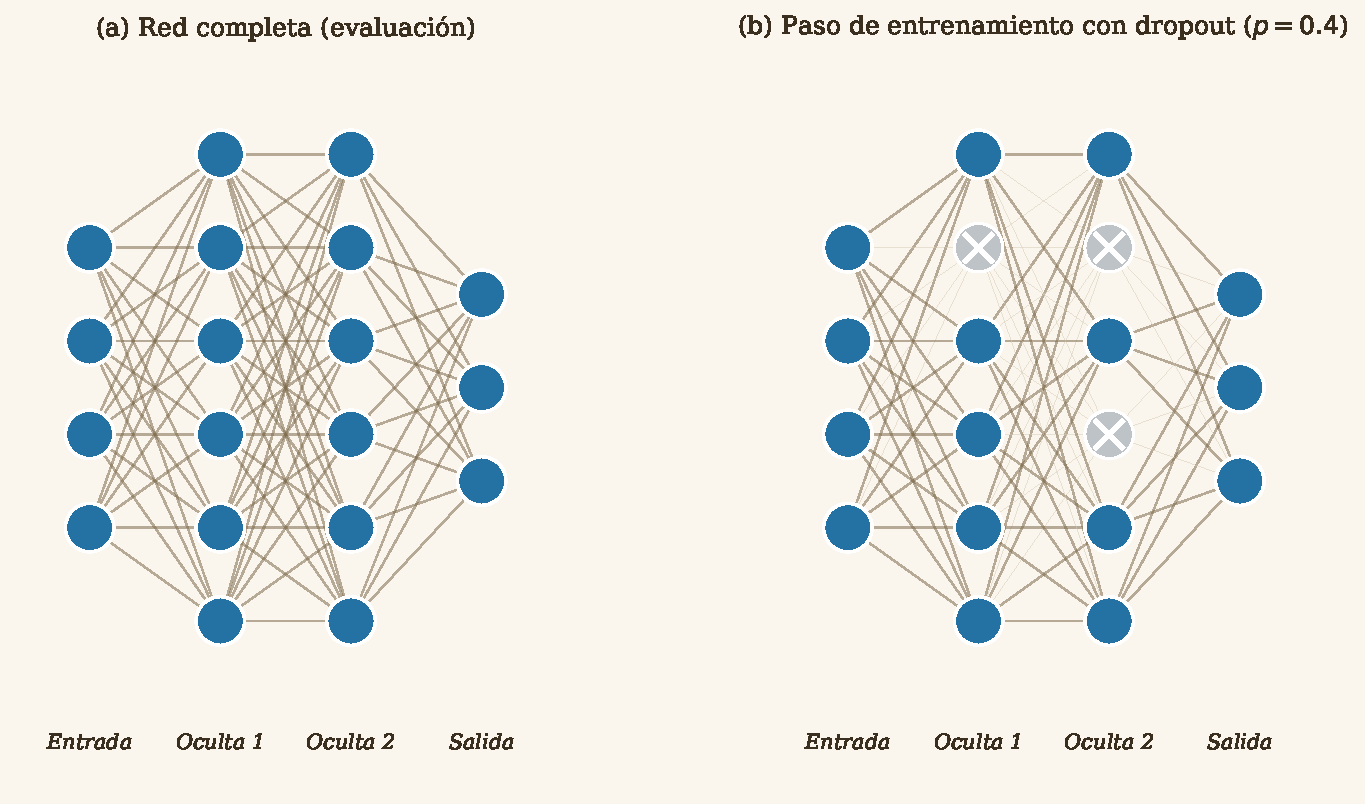
\includegraphics[width=0.95\textwidth]{figuras/figura_dropout}
  \caption[Mecanismo de \textit{dropout} durante el entrenamiento]{\textbf{Mecanismo de \textit{dropout} durante el entrenamiento.} (a) Red neuronal completa (\textit{fully connected}) durante la fase de inferencia o evaluación, donde todas las unidades están activas. (b) La misma red durante un paso de entrenamiento con \textit{dropout} ($p=0.4$); un subconjunto aleatorio de neuronas (en gris claro) y sus conexiones asociadas se desactivan. Esto obliga a la red a aprender representaciones más robustas y redundantes, reduciendo significativamente el sobreajuste.}
  \label{fig:dropout}
\end{figure}

\subsection{Desbalance de clases: \textit{pos\_weight} y \textit{Focal Loss}}
\label{desbalance}

El pronóstico sísmico es un problema fuertemente desbalanceado: en California y Alaska entre 2000 y 2024, sólo el $\sim 30\%$ de los días tienen al menos un \textit{mainshock} $M\geq 4.5$ en los siguientes \(30\) días; en una formulación por celda el ratio cae a $\sim 2\%$ \citep{he2009imbalanced}. Para mitigarlo se utiliza:
\begin{enumerate}
  \item \textbf{Ponderación de clase} (\textit{pos\_weight} en \texttt{BCEWithLogitsLoss}): asigna un peso $w_+ = N_-/N_+$ a la clase minoritaria.
  \item \textbf{\textit{Focal Loss}} \citep{lin2017focal}: \(\mathrm{FL}(p_t) = -\alpha_t\, (1 - p_t)^\gamma\, \log p_t\), que reduce el peso de los ejemplos fáciles ($p_t$ cercano a 1) y enfatiza los difíciles. Con $\gamma=2$ se obtiene típicamente mejor desempeño en problemas con desbalance fuerte.
\end{enumerate}

\section{Arquitecturas para series temporales}
\label{dl-temporal}

\subsection{Redes recurrentes y LSTM}

Las redes recurrentes (\gls{rnn}) procesan secuencias actualizando un estado oculto a cada paso temporal. La variante \emph{Long Short-Term Memory} (\gls{lstm}) de \citet{hochreiter1997lstm} introduce un mecanismo de \textit{gates} (\textit{forget gate}, \textit{input gate}, \textit{output gate}) que mitiga el problema del gradiente desvaneciente, permitiendo aprender dependencias de varias decenas a centenas de pasos. Han sido la arquitectura dominante en series temporales durante la década 2010--2020. Sus limitaciones --paralelización difícil, \textit{receptive field} efectivo limitado-- motivan las alternativas que se discuten a continuación.

\subsection{Temporal Convolutional Networks}
\label{tcn-marco}

Las \emph{Temporal Convolutional Networks} (\gls{tcn}), introducidas por \citet{bai2018tcn}, sustituyen la recurrencia por una pila de convoluciones 1D \emph{causales} y \emph{dilatadas} con conexiones residuales. Sus tres características definitorias son:

\begin{itemize}
  \item \textbf{Causalidad:} la salida en el tiempo $t$ depende solamente de las entradas en $t' \leq t$ (la convolución está desplazada para no usar el futuro).
  \item \textbf{Dilataciones exponenciales:} la $\ell$-ésima capa usa dilatación $d_\ell = 2^{\ell - 1}$, lo que permite un \emph{receptive field} (RF) que crece exponencialmente con la profundidad según
        \begin{equation}
          \mathrm{RF} = 1 + 2\,(K-1)\,(2^L - 1),
          \label{eq:rf-tcn}
        \end{equation}
        donde $K$ es el tamaño del \textit{kernel} y $L$ el número de capas. Para $K=3$, $L=4$ se obtiene RF $=61$, que cubre una ventana de aproximadamente dos meses (con resolución diaria) y motiva la elección del \texttt{LOOKBACK $=60$ días} en este trabajo.
  \item \textbf{Bloques residuales:} cada bloque añade un atajo $h \mapsto h + \mathrm{conv}(h)$ que facilita el entrenamiento de redes profundas.
\end{itemize}

Se mostraron empíricamente que las TCN igualan o superan a las LSTM en una amplia batería de benchmarks de modelado de secuencias (véase Tabla~\ref{tab:tcn-vs-lstm} en el Anexo~\ref{anexo-tcn-lstm}), con la ventaja adicional de la paralelización por GPU. Esto las hace candidatas naturales para modelar series temporales de sismicidad con resolución diaria, como se hace en el capítulo \ref{desarrollo-del-proyecto-y-resultados}.

\begin{figure}[ht!]
  \centering
  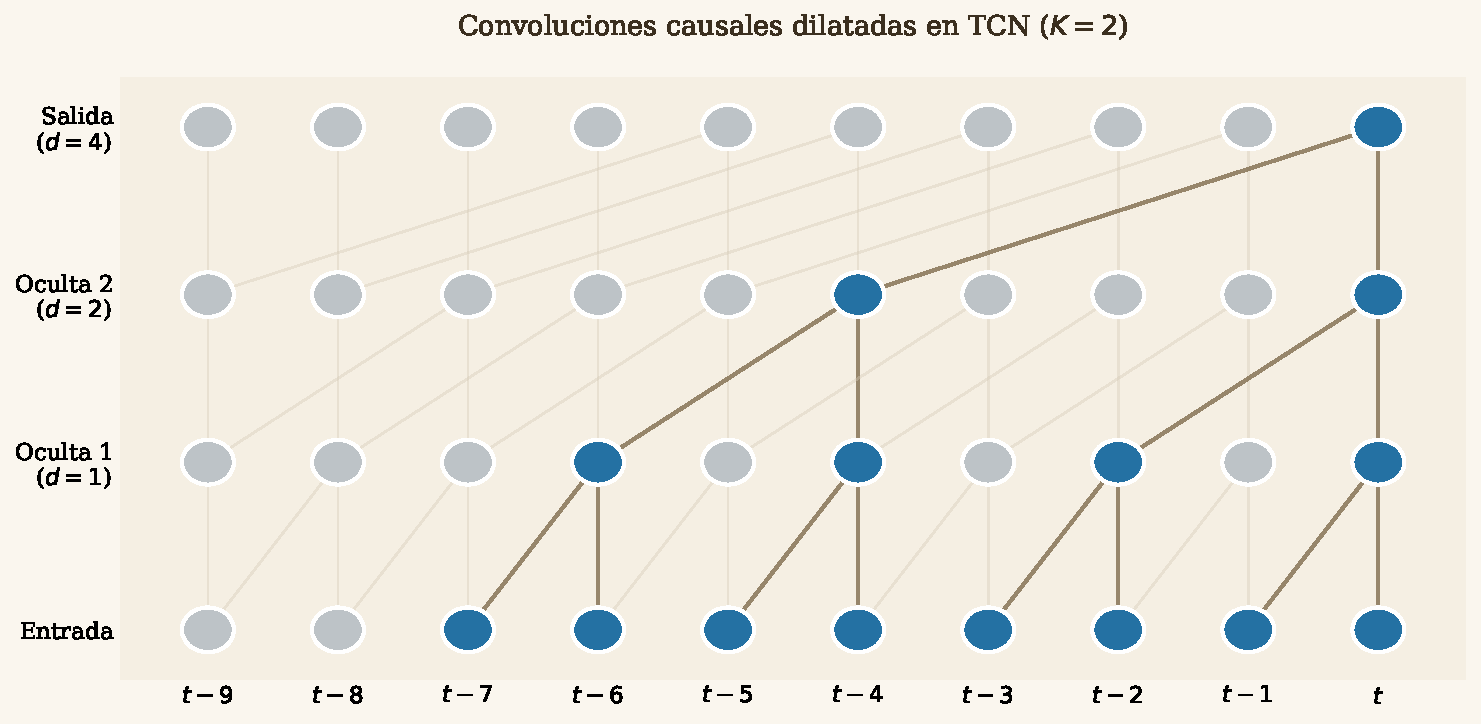
\includegraphics[width=0.9\textwidth]{figuras/figura_tcn}
  \caption[Arquitectura de una \textit{Temporal Convolutional Network} (TCN)]{\textbf{Convoluciones causales dilatadas en una TCN.} Ilustración del mecanismo para $K=2$ y dilataciones $d=\{1, 2, 4\}$. La causalidad asegura que no haya fuga de información del futuro, y las dilataciones exponenciales permiten que el \textit{receptive field} crezca rápidamente con la profundidad de la red, capturando dependencias a largo plazo de manera eficiente. Figura inspirada en \citet{bai2018tcn}.}
  \label{fig:tcn}
\end{figure}

\subsection{Mecanismo de atención y Transformers}

\citet{vaswani2017attention} propusieron el \emph{Transformer}, basado íntegramente en \emph{atención} sobre la secuencia sin recurrencia ni convolución. El cálculo de la atención mediante producto punto escalar se define como
\begin{equation}
  \mathrm{Attn}(Q, K, V) = \mathrm{softmax}\!\left(\frac{QK^\top}{\sqrt{d_k}}\right) V,
  \label{eq:attention}
\end{equation}
donde $Q, K, V$ son las proyecciones \emph{query, key, value} de la entrada. Su capacidad para modelar dependencias arbitrariamente largas en paralelo lo ha convertido en la arquitectura dominante en el procesamiento del lenguaje natural (NLP), la visión y, más recientemente, la sismología (EQTransformer \citep{mousavi2020eqtransformer}). En este trabajo se utiliza tanto el Transformer indirectamente (vía EQTransformer preentrenado en el notebook 02) como directamente bajo la forma de \emph{Transformer con codificación geoespacial} sobre la red de celdas activas.

\section{Arquitecturas para datos estructurados en grafo}
\label{dl-grafos}

\subsection{Motivación geofísica}

La sismicidad regional tiene una estructura espacial naturalmente representable como grafo: cada estación (o cada celda de discretización) es un nodo, y existen \emph{relaciones} físicamente significativas entre nodos cercanos (transferencia de estrés de Coulomb, propagación de ondas, conectividad de fallas). Las \gls{gnn} \citep{scarselli2009gnn} generalizan el operador convolucional a grafos arbitrarios y son por tanto la arquitectura natural para esta representación.

\subsection{Graph Convolutional Networks (GCN)}
\label{gcn-marco}

\citet{kipf2017gcn} introdujeron la \gls{gcn}, cuya capa se define como
\begin{equation}
  H^{(\ell+1)} = \sigma\!\left(\tilde{D}^{-\frac{1}{2}}\, \tilde{A}\, \tilde{D}^{-\frac{1}{2}}\, H^{(\ell)}\, W^{(\ell)}\right),
  \label{eq:gcn}
\end{equation}
donde $\tilde{A} = A + I$ es la matriz de adyacencia con autoaristas (\textit{self-loops}), $\tilde{D}$ su matriz de grados, $H^{(\ell)}$ las representaciones de los nodos en la capa $\ell$, $W^{(\ell)}$ los pesos aprendibles y $\sigma$ una no linealidad. La normalización simétrica $\tilde{D}^{-1/2}\tilde{A}\tilde{D}^{-1/2}$ asegura estabilidad numérica y un espectro acotado del operador de propagación.

El significado intuitivo es que cada nodo agrega información de sus vecinos inmediatos, ponderada por el grado, antes de aplicar una transformación lineal. Apilando $L$ capas, un nodo recibe información de su entorno $L$-saltos. En el modelo propuesto en el capítulo \ref{desarrollo-del-proyecto-y-resultados}, se utiliza una variante \emph{spatiotemporal} en la que una TCN comparte pesos entre celdas para procesar la dimensión temporal y a continuación dos capas GCN propagan información espacial entre celdas.

\subsection{Graph Attention Networks (GAT)}
\label{gat-marco}

\citet{velickovic2018gat} propusieron las \emph{Graph Attention Networks} (\gls{gat}), que sustituyen la ponderación fija del grado por una atención aprendible entre cada par de nodos vecinos:
\begin{equation}
  \alpha_{ij} = \frac{\exp\!\left(\mathrm{LeakyReLU}(\mathbf{a}^\top [W h_i \| W h_j])\right)}{\sum_{k \in \mathcal{N}(i)} \exp\!\left(\mathrm{LeakyReLU}(\mathbf{a}^\top [W h_i \| W h_k])\right)},
\end{equation}
donde $\mathbf{a}$ es un vector aprendible y $\|$ denota concatenación. GAT ofrece interpretabilidad (qué vecinos pesan más) a costa de un número mayor de parámetros. En este trabajo se utiliza GCN como arquitectura principal y se reserva GAT como ablation futura.

\subsection{Construcción del grafo: distancia de Haversine y \textit{KNN fallback}}

El grafo entre celdas activas se construye conectando pares cuya distancia de Haversine
\begin{equation}
  d(\mathbf{p}_1, \mathbf{p}_2) = 2 R\, \mathrm{arc\,sen}\!\left(\sqrt{\sin^2\!\tfrac{\Delta\varphi}{2} + \cos\varphi_1\,\cos\varphi_2\,\sin^2\!\tfrac{\Delta\lambda}{2}}\right),
  \label{eq:haversine}
\end{equation}
es menor que un umbral (\(100\) km en este trabajo). En la expresión, $\mathbf{p}_1$ y $\mathbf{p}_2$ son los centroides de las dos celdas; $\varphi$ denota la \emph{latitud} y $\lambda$ la \emph{longitud} de cada punto (en radianes), de modo que $\varphi_1,\varphi_2$ son las latitudes respectivas, $\Delta\varphi = \varphi_2 - \varphi_1$ la diferencia de latitud y $\Delta\lambda = \lambda_2 - \lambda_1$ la de longitud; $R$ es el radio medio de la Tierra ($\approx 6371$\,km). Para garantizar que ningún nodo quede aislado se aplica un \textit{fallback} basado en los K vecinos más cercanos (KNN, $k=2$) que conecta cada nodo a sus dos vecinos más cercanos aunque excedan el umbral. Esta combinación garantiza grado mínimo $\geq 2$ sin perder estructura física.

\subsection{Software: PyTorch Geometric}

La implementación de GNNs en este trabajo se apoya en \emph{PyTorch Geometric} \citep{fey2019pyg}, librería estandarizada para grafos sobre \emph{PyTorch} \citep{paszke2019pytorch}. PyG proporciona implementaciones eficientes de GCN, GAT y otros operadores, y simplifica la gestión de batches de grafos heterogéneos.

\section{Cuantificación de incertidumbre: Procesos Gaussianos}
\label{dl-incertidumbre}

Una predicción probabilística de riesgo sísmico tiene poca utilidad operativa si no viene acompañada de una estimación de su incertidumbre. Los \emph{Procesos Gaussianos} (\gls{gp}, \citep{rasmussen2006gp}) son un marco bayesiano no paramétrico ideal para esta tarea: definen una distribución de probabilidad sobre funciones $f \sim \mathcal{GP}(m, k)$, especificada por una función de media $m(\mathbf{x})$ y un \textit{kernel} de covarianza $k(\mathbf{x}, \mathbf{x}')$. Dado un conjunto de observaciones $\{(\mathbf{x}_i, y_i)\}$, la predicción posterior es nuevamente Gaussiana con media y varianza analíticas:
\begin{align}
  \mu_*(\mathbf{x}_*)      & = \mathbf{k}_*^\top (K + \sigma_n^2 I)^{-1} \mathbf{y},                                   \\
  \sigma_*^2(\mathbf{x}_*) & = k(\mathbf{x}_*, \mathbf{x}_*) - \mathbf{k}_*^\top (K + \sigma_n^2 I)^{-1} \mathbf{k}_*,
\end{align}
con $K_{ij} = k(\mathbf{x}_i, \mathbf{x}_j)$ y $\mathbf{k}_* = [k(\mathbf{x}_*, \mathbf{x}_i)]_i$. La elección del \textit{kernel} codifica las hipótesis a priori sobre la suavidad y la escala característica del fenómeno. Para datos sísmicos espaciales se utilizan típicamente \textit{kernels} de tipo Matérn con escalas de varios kilómetros.

En el sistema integrado propuesto, el GP recibe como entrada las probabilidades brutas $\hat{p}(\text{\emph{celda}}, \text{\emph{día}})$ generadas por la GNN y produce un campo suave $(\mu_*, \sigma_*)$ que constituye el mapa final de riesgo. Esto combina la potencia representacional del aprendizaje profundo (DL) con la estricta cuantificación bayesiana del GP.

\section{Mapas de peligrosidad y riesgo sísmico}
\label{mapas-riesgo}

\subsection{Peligro, exposición, vulnerabilidad y riesgo}
En el ámbito de la sismología aplicada y la ingeniería sísmica, resulta fundamental establecer una demarcación terminológica rigurosa entre cuatro conceptos interdependientes. El \emph{peligro sísmico} (\textit{seismic hazard}) denota la probabilidad de que ocurra un evento de cierta intensidad en un emplazamiento y periodo de tiempo definidos. La \emph{exposición} refiere al inventario de elementos físicos o humanos (población, infraestructuras) situados en la zona de afectación. La \emph{vulnerabilidad} cuantifica la susceptibilidad de dichos elementos a sufrir daños frente a un determinado nivel de sacudida. Finalmente, el \emph{riesgo sísmico} (\textit{seismic risk}) es la convolución matemática de los tres factores anteriores, estimando las pérdidas potenciales (económicas o humanas). El alcance computacional y metodológico de este TFM se centra exclusivamente en el modelado del \emph{peligro}, aunque sus resultados sirven de base fundamental para cualquier análisis de riesgo posterior.

\subsection{PSHA (\textit{Probabilistic Seismic Hazard Assessment}) vs. OEF}
La evaluación del peligro sísmico se ha regido históricamente por el paradigma PSHA, introducido formalmente por \citet{cornell1968engineering} y estandarizado metodológicamente por \citet{mcguire1995probabilistic}. Este enfoque clásico persigue la estimación probabilística de la tasa de excedencia de diferentes niveles de aceleración del terreno a largo plazo (típicamente horizontes de 50 años), asumiendo un modelo estadístico subyacente de Poisson (es decir, una tasa de sismicidad constante e independiente de la historia reciente).

En contraste directo con esta perspectiva estática a largo plazo, el Pronóstico Operacional de Terremotos (\textit{Operational Earthquake Forecasting}, OEF) \citep{jordan2011oef} aborda las fluctuaciones espaciotemporales dinámicas de la sismicidad a muy corto plazo (días o semanas). Dado que el marco temporal de predicción propuesto en este TFM opera sobre ventanas prospectivas de 30 días apoyadas en aprendizaje profundo, el sistema desarrollado se categoriza conceptualmente dentro del paradigma dinámico OEF, suplementando, pero no sustituyendo, a los mapas estáticos PSHA tradicionales.

\subsection{De probabilidad por celda a mapa continuo}
Los algoritmos de clasificación de aprendizaje automático, especialmente aquellos operando sobre una discretización espacial (rejilla o \textit{grid}), devuelven típicamente una variable de salida logística (pseudoprobabilidad) asociada al centroide de cada celda. Para que estas inferencias brutas adquieran la categoría de mapa de peligrosidad accionable, requieren dos etapas de posprocesamiento (véase la Figura~\ref{fig:mapa-riesgo}).

En primera instancia, las puntuaciones deben ser calibradas probabilísticamente para asegurar que reflejan tasas de ocurrencia empíricas reales. Métodos de calibración como el escalado de Platt \citep{platt1999probabilistic} o la regresión isotónica mapean las salidas de los márgenes del clasificador hacia probabilidades matemáticas condicionales estrictas. En segunda instancia, el mapa de probabilidades por celda discreta debe ser interpolado espacialmente (e.g., \textit{kriging} universal). Es en esta etapa de interpolación topológica continua donde los Procesos Gaussianos (véase \ref{dl-incertidumbre}) evidencian su utilidad práctica, generando una superficie analítica suave que incluye bandas de confianza para cada coordenada geoespacial.

\begin{figure}[ht!]
  \centering
  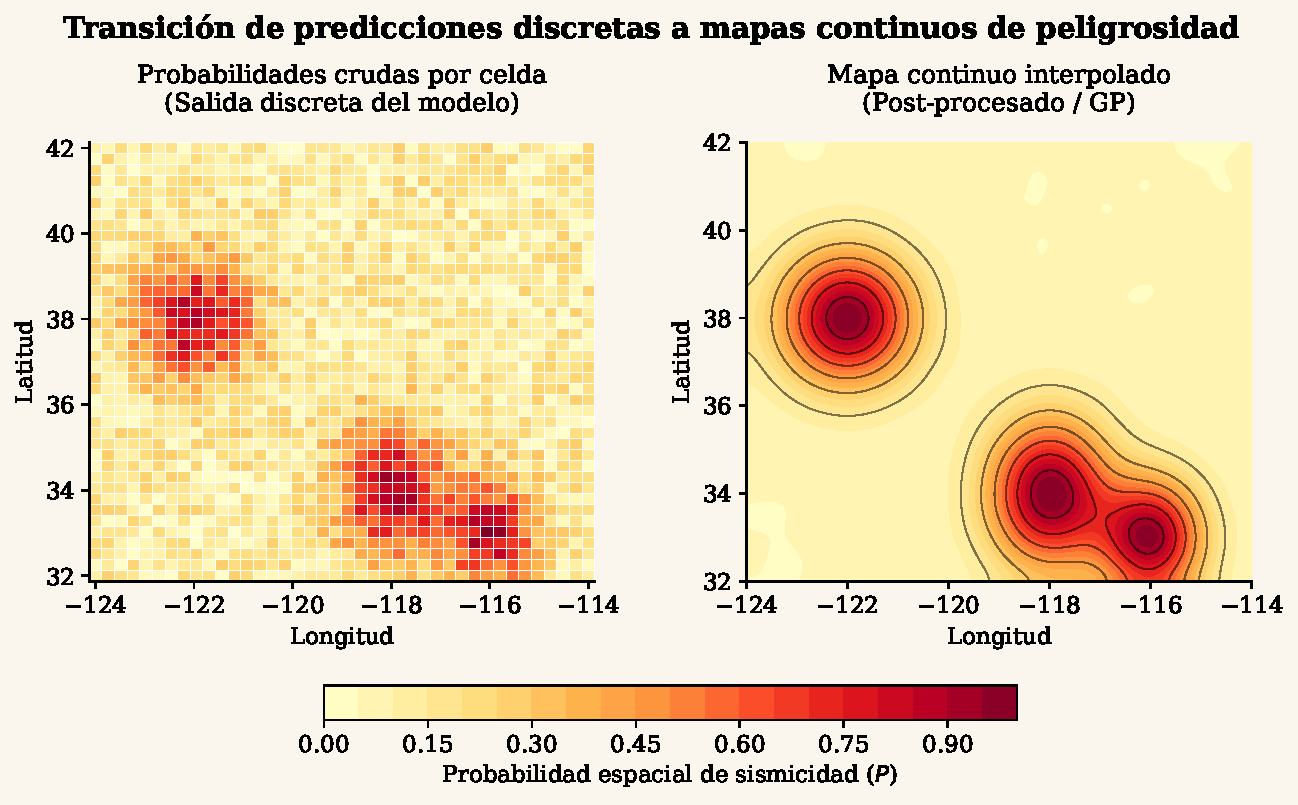
\includegraphics[width=0.9\textwidth]{figuras/figura_mapa_riesgo}
  \caption[Transición de predicciones discretas a mapas continuos de peligrosidad]{\textbf{Transición de predicciones discretas a mapas continuos de peligrosidad.} Izquierda: Probabilidades brutas (\textit{raw}) emitidas por un modelo de inferencia operando sobre una partición espacial discreta. Derecha: Superficie de peligrosidad interpolada mediante posprocesamiento espacial continuo (e.g., Procesos Gaussianos), donde se delinean isolíneas que demarcan frentes equiprobables, un formato mucho más asimilable para la gestión de emergencias.}
  \label{fig:mapa-riesgo}
\end{figure}

\subsection{Visualización y comunicación}
El diseño de mapas de riesgo sísmico debe priorizar la claridad y facilidad de comprensión tanto para los gestores de protección civil como para el público general. Herramientas de referencia en la ingeniería geofísica como \emph{ShakeMap} \citep{wald1999shakemap} han fijado los estándares en el uso de paletas de color y curvas de nivel (isolíneas) para representar con precisión la intensidad del movimiento del suelo. Asimismo, proyectos centrados en fallas a gran escala, como el modelo californiano UCERF3 \citep{field2014ucerf3}, basan sus metodologías de difusión en este mismo tipo de visualizaciones cartográficas. Este enfoque de comunicación transparente y estandarizada responde directamente a los principios éticos de difusión del riesgo promovidos por el Marco de Sendai \citep{un2015sendai}.

\section{Aprendizaje profundo aplicado a sismología}
\label{dl-sismologia}

\subsection{Detección y \textit{picking}: PhaseNet, EQTransformer y GPD}
\label{deteccion-picking}

\citet{zhu2018phasenet} introdujeron \emph{PhaseNet}, una U-Net 1D entrenada sobre $\sim 700\,000$ formas de onda etiquetadas para identificar y localizar las llegadas P y S. Cada traza de tres componentes a 100\,Hz se procesa por una red en forma de ``U'' con saltos simétricos y produce tres canales de salida: probabilidad de P, probabilidad de S y probabilidad de ruido. Sus errores de \textit{picking} son comparables a los de un analista humano y su \emph{recall} supera ampliamente al de los métodos heurísticos tipo STA/LTA.

\citet{mousavi2020eqtransformer} propusieron \emph{EQTransformer}, una red que ha pasado a ser una de las herramientas más usadas en sismología moderna. La idea principal es resolver tres tareas a la vez con un solo modelo: decir si hay un terremoto en el registro, marcar la llegada de la onda P y marcar la llegada de la onda S. Para ello combina tres ingredientes que ya habían funcionado por separado en otros trabajos pero que aquí se integran por primera vez:

\begin{enumerate}
  \item Una \textbf{parte convolucional} (CNN, \textit{Convolutional Neural Network}) que actúa como ``ojo'' inicial y extrae características locales del sismograma, parecido a cómo un humano se fija en la forma de los picos y los cambios bruscos.
  \item Una \textbf{parte recurrente bidireccional} (BiLSTM, \textit{Bidirectional LSTM}) que recorre la señal hacia delante y hacia atrás, recordando lo que ha pasado antes y después de cada instante para no descartar información que solo es útil al ver el contexto completo.
  \item Un \textbf{mecanismo de atención} de tipo \textit{Transformer} que aprende, por sí solo, qué fragmentos del sismograma son los más informativos para cada tarea y los ``ilumina'' frente al resto. Este es el componente que da nombre a la red y la diferencia de PhaseNet: en lugar de mirar la traza con la misma resolución en todas partes, el modelo decide dónde concentrar el cómputo.
\end{enumerate}

La red está entrenada sobre \gls{stead} con etiquetas precisas de llegada P y S, y devuelve tres canales de probabilidad sincronizados (detección, P, S) que se leen como funciones del tiempo. Cuando uno de esos canales supera un umbral configurable, se considera una predicción. En las pruebas originales sobre el propio STEAD y sobre datos no vistos de la red sísmica del norte de California, EQTransformer iguala o mejora a PhaseNet en \textit{recall} y comete menos falsos positivos en presencia de ruido o de eventos solapados, gracias al efecto regularizador del mecanismo de atención. Además, la versión preentrenada generaliza razonablemente bien a regiones distintas a las del entrenamiento. Por todas estas razones se ha convertido, junto con PhaseNet, en uno de los dos modelos de referencia para detección y \textit{picking} automáticos y es la única arquitectura que, en una sola pasada, cubre las tres tareas más comunes del pipeline sismológico.

\begin{figure}[ht!]
  \centering
  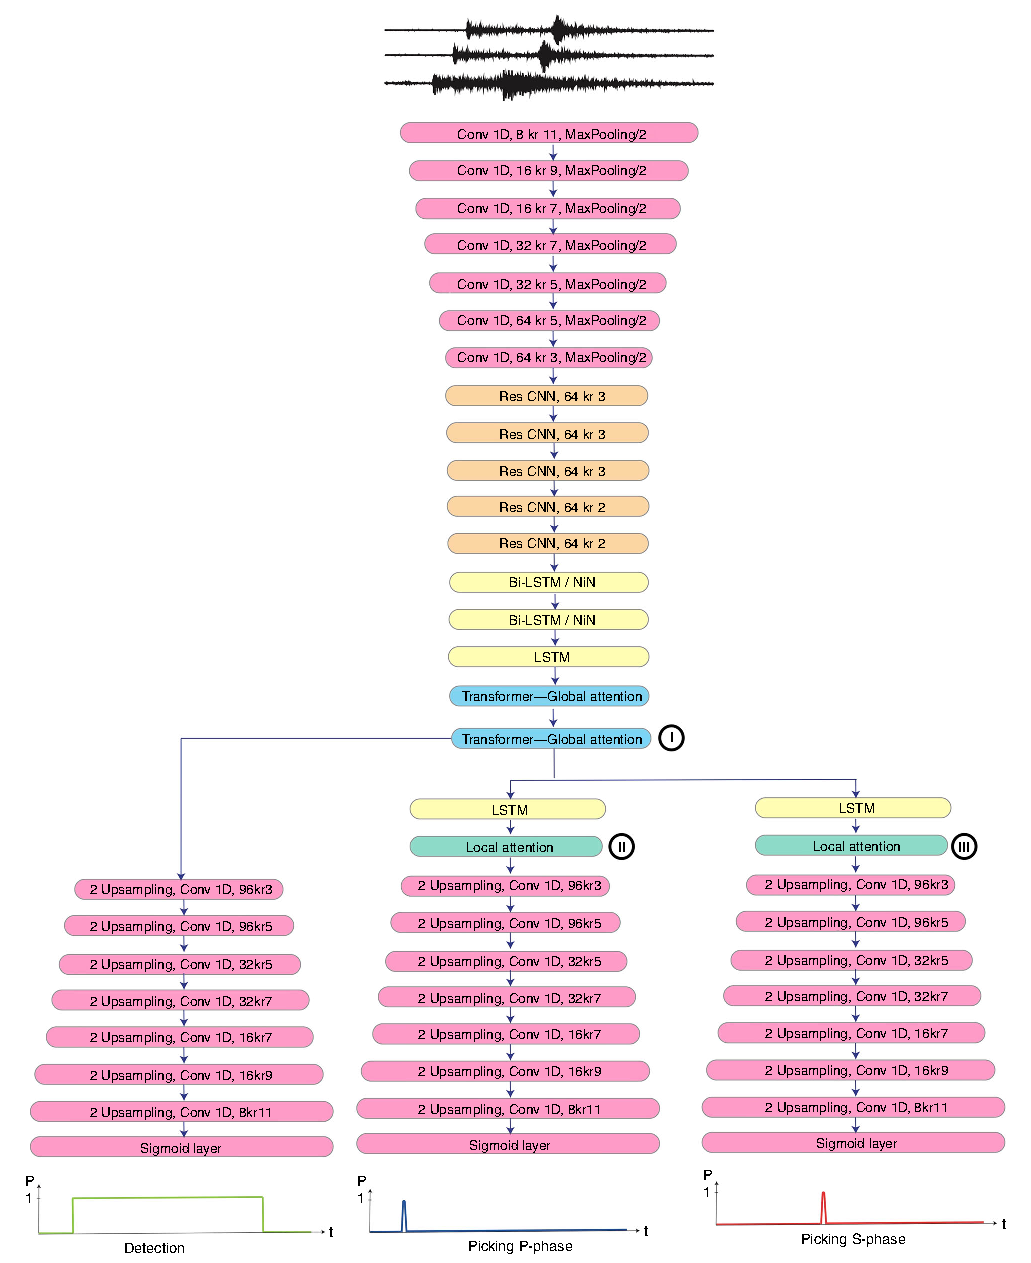
\includegraphics[width=0.8\textwidth]{figuras/figura_eqtransformer}
  \caption[Arquitectura de EQTransformer \citep{mousavi2020eqtransformer}]{\textbf{Arquitectura de EQTransformer \citep{mousavi2020eqtransformer}.} El sismograma de tres componentes (6000 muestras, 60\,s a 100\,Hz) entra por la parte superior y se procesa mediante bloques convolucionales y mecanismos de atención para detectar eventos sísmicos y estimar las llegadas de ondas P y S.}
  \label{fig:eqtransformer}
\end{figure}

Adicionalmente, \citet{ross2018generalized} mostraron con \emph{Generalized Phase Detection} (GPD) la viabilidad de una CNN simple entrenada en California que generaliza bien a otras regiones, y \citet{perol2018convnetquake} demostraron en \emph{Science Advances} que una CNN puede detectar y localizar simultáneamente eventos en Oklahoma. \citet{mousavi2019cred} añadieron \emph{CRED}, un modelo residual híbrido CNN + RNN para detección con baja relación señal-ruido (SNR). Todas estas arquitecturas están accesibles a través de \emph{SeisBench} \citep{woollam2022seisbench}, un toolkit estandarizado para aprendizaje automático (ML) en sismología que se usa en este trabajo (notebook 02).

\subsection{Pronóstico y detección de precursores}
\label{pronostico-precursores}

\citet{devries2018aftershocks} publicaron en \emph{Nature} una red densa que predice la distribución espacial de réplicas a partir de métricas de transferencia de estrés; aunque su evaluación inicial fue cuestionada posteriormente, abrió la línea de pronóstico espacial con DL. \citet{rouetleroy2017slowslip} aplicaron \emph{Random Forests} sobre señales acústicas en laboratorio para predecir deslizamientos en fallas controladas, mostrando que la señal estacional de \textit{slip} contiene información precursora explotable. \citet{vandenende2024forecasting} extendieron muy recientemente esta línea a \emph{deep neural temporal point processes} sobre catálogos reales, mostrando ganancias significativas sobre ETAS.

Para la \textbf{asociación de fases en redes densas}, \citet{mcbrearty2023gnn} desarrollaron una GNN específica que demuestra que la estructura de grafo natural de la red de estaciones puede explotarse para asociar correctamente picks pertenecientes al mismo evento, problema que tradicionalmente requería heurísticas complejas. Para la \textbf{caracterización automática de fuentes} (mecanismo focal, momento sísmico), \citet{vandenende2020tcnseismic} aplicaron GNNs sobre las formas de onda registradas en múltiples estaciones de la misma red.

\subsection{Revisiones del campo}

Las revisiones recientes más relevantes son \citet{kong2019mlseismology} en \emph{SRL}, \citet{beroza2021dlreview} en \emph{Nature Communications} y la más reciente \citet{mousavi2023review} en \emph{Annual Review of Earth and Planetary Sciences}. Las tres coinciden en señalar que el campo ha madurado en detección y \textit{picking} (PhaseNet/EQT como estándar de facto), pero todavía se encuentra en una fase inicial en pronóstico y predicción, donde la mayor parte de la mejora ha venido de un manejo más cuidadoso de los datos y los \textit{baselines} más que de cambios fundamentales de arquitectura.

\section{Métricas de evaluación en escenarios de desbalance extremo}
\label{metricas-desbalance}

\subsection{La paradoja del \textit{accuracy}}
\label{paradoja-accuracy}

En problemas de clasificación con clases muy desequilibradas, como el pronóstico sísmico, la métrica más intuitiva --el porcentaje de aciertos o \textit{accuracy}-- se vuelve engañosa. En este TFM, por ejemplo, los días con un \textit{mainshock} $M\geq 4.5$ en los siguientes 30 días representan en torno al 30\,\% del total a escala global y caen por debajo del 2\,\% cuando el problema se formula por celda. Un modelo que predijera ``no habrá terremoto'' de forma constante alcanzaría entre un 70 y un 98\,\% de \textit{accuracy} sin aportar nada útil. Para evitar esta trampa se utilizan métricas que separan los aciertos por clase y penalizan tanto los falsos positivos como los falsos negativos \citep{he2009imbalanced}.

\subsection{Precision, recall y F1-score}
\label{precision-recall-f1}

A partir de la matriz de confusión, con TP (verdaderos positivos), FP (falsos positivos), TN (verdaderos negativos) y FN (falsos negativos), se definen las dos métricas básicas
\begin{equation}
  \mathrm{Precision} = \frac{TP}{TP + FP}, \qquad \mathrm{Recall} = \frac{TP}{TP + FN}
  \label{eq:precision-recall}
\end{equation}
y su media armónica, el \textit{F1-score}
\begin{equation}
  F_1 = 2 \cdot \frac{\mathrm{Precision} \cdot \mathrm{Recall}}{\mathrm{Precision} + \mathrm{Recall}}
  \label{eq:f1}
\end{equation}

\textit{Recall} responde a la pregunta ``de los terremotos que realmente ocurrieron, ¿cuántos consiguió detectar el modelo?'', mientras que \textit{Precision} responde a ``de las alarmas que el modelo emitió, ¿cuántas correspondieron a un terremoto real?''. Ambas métricas están en tensión: subir el umbral de decisión mejora la \textit{Precision} a costa del \textit{Recall}, y viceversa. El F1-score resume el equilibrio entre las dos en un único número.

En un sistema operativo de pronóstico, qué métrica priorizar depende del coste relativo de cada tipo de error. Un alto \textit{Recall} es esencial cuando perderse un terremoto es inaceptable (alerta temprana en zonas pobladas), mientras que una alta \textit{Precision} se prefiere cuando las falsas alarmas tienen un coste social o económico relevante (evacuaciones, parones industriales).

\subsection{Curva Precision-Recall y PR-AUC}
\label{pr-auc}

La curva ROC, que enfrenta la tasa de verdaderos positivos contra la de falsos positivos, es la métrica más conocida en aprendizaje automático y la que reportamos como AUC en la sección de metodología. Sin embargo, cuando la clase positiva es muy minoritaria, la curva ROC tiene un sesgo bien documentado: la tasa de falsos positivos queda artificialmente baja porque el denominador (los negativos) es enorme, lo que hace que cualquier modelo deficiente produzca una curva visualmente convincente \citep{davis2006relationship, saito2015precision}.

La alternativa estándar es la curva \textbf{Precision-Recall} y su área bajo la curva, la \textbf{PR-AUC}. A diferencia de la ROC, la PR-AUC ignora los verdaderos negativos (mayoritarios y poco informativos) y refleja directamente el rendimiento sobre la clase de interés. La línea base de la PR-AUC no es 0.5 como en la ROC del modelo aleatorio, sino el ratio de positivos del problema; en nuestra formulación por celda, una PR-AUC de aproximadamente 0.02 sería el suelo correspondiente al modelo aleatorio. \citet{saito2015precision} muestran empíricamente que la PR-AUC discrimina mejor entre clasificadores cuando el desbalance supera 1:10, y es la métrica que las revistas Q1 del área tienden a exigir cuando la clase positiva es rara \citep{davis2006relationship}.

\subsection{Diagrama de Molchan}
\label{molchan}

La sismología cuenta con una métrica propia diseñada específicamente para evaluar predicciones de tipo ``alarma'': el \textbf{diagrama de Molchan}, propuesto por \citet{molchan1991structure} y formalizado para el programa CSEP (\textit{Collaboratory for the Study of Earthquake Predictability}) por \citet{zechar2008testing}. El diagrama mide el rendimiento de un sistema de pronóstico mediante dos magnitudes:

\begin{itemize}
  \item $\nu$ (\textit{miss rate}): fracción de terremotos reales que el modelo \emph{no} consiguió alertar.
  \item $\tau$ (\textit{fraction of space-time covered by alarm}): fracción del volumen espacio-temporal total que el modelo declaró en estado de alarma.
\end{itemize}

Cada punto del diagrama representa un par $(\tau, \nu)$ asociado a un umbral de decisión concreto. Un modelo aleatorio queda sobre la diagonal $\nu = 1 - \tau$; cualquier modelo con habilidad real cae por debajo de esa línea. El área entre la curva y la diagonal es una medida resumen del \textit{skill} del pronosticador, conceptualmente análoga a la PR-AUC pero adaptada a la geometría espacio-temporal del problema sísmico.

La ventaja del diagrama de Molchan respecto a las métricas estándar de aprendizaje automático es triple. En primer lugar, separa explícitamente la dimensión espacial de la temporal: un modelo que cubriera todo el territorio durante el 100\,\% del tiempo nunca fallaría un terremoto, pero su $\tau = 1$ lo descartaría como pronosticador útil. En segundo lugar, permite comparar de forma directa con sistemas operativos como UCERF3-ETAS \citep{field2017ucerf3etas} o el OEF italiano \citep{marzocchi2014oef}, que reportan sus resultados en este formato. Y en tercer lugar, es la métrica de referencia exigida por CSEP, la infraestructura internacional que centraliza la validación experimental de pronósticos sísmicos \citep{zechar2008testing}.

En este TFM se reportarán, además de la AUC y la PR-AUC, las curvas de Molchan correspondientes a cada modelo, lo que permitirá una comparación directa con la literatura sismológica de referencia.

\section{Datasets de referencia: STEAD}
\label{stead}

El \emph{STanford EArthquake Dataset} (STEAD) \citep{mousavi2019stead} es en la actualidad el catálogo público de formas de onda sísmicas más extenso y accesible. Constituye el estándar de referencia (\emph{benchmark}) fundamental para el entrenamiento y la evaluación comparativa de modelos de aprendizaje profundo en sismología. En total, incluye más de $1.2$ millones de trazas sísmicas. Cada uno de estos registros tiene una duración de $60$ segundos y contiene mediciones en tres componentes espaciales: Este, Norte y Vertical (E, N, Z). Con una frecuencia de muestreo de $100$\,Hz, cada registro consta de $6\,000$ observaciones discretas por componente.

Los datos provienen de redes sismológicas distribuidas a nivel global, abarcando eventos registrados entre 1984 y 2018. La casuística contemplada incluye desde microseísmos (magnitud $-0.5$) hasta sismos de gran escala (magnitud $7.9$), detectados a distancias hipocentrales que oscilan entre $0$ y $350$ kilómetros (véase la Figura~\ref{fig:histograma-stead}).

\begin{figure}[ht!]
  \centering
  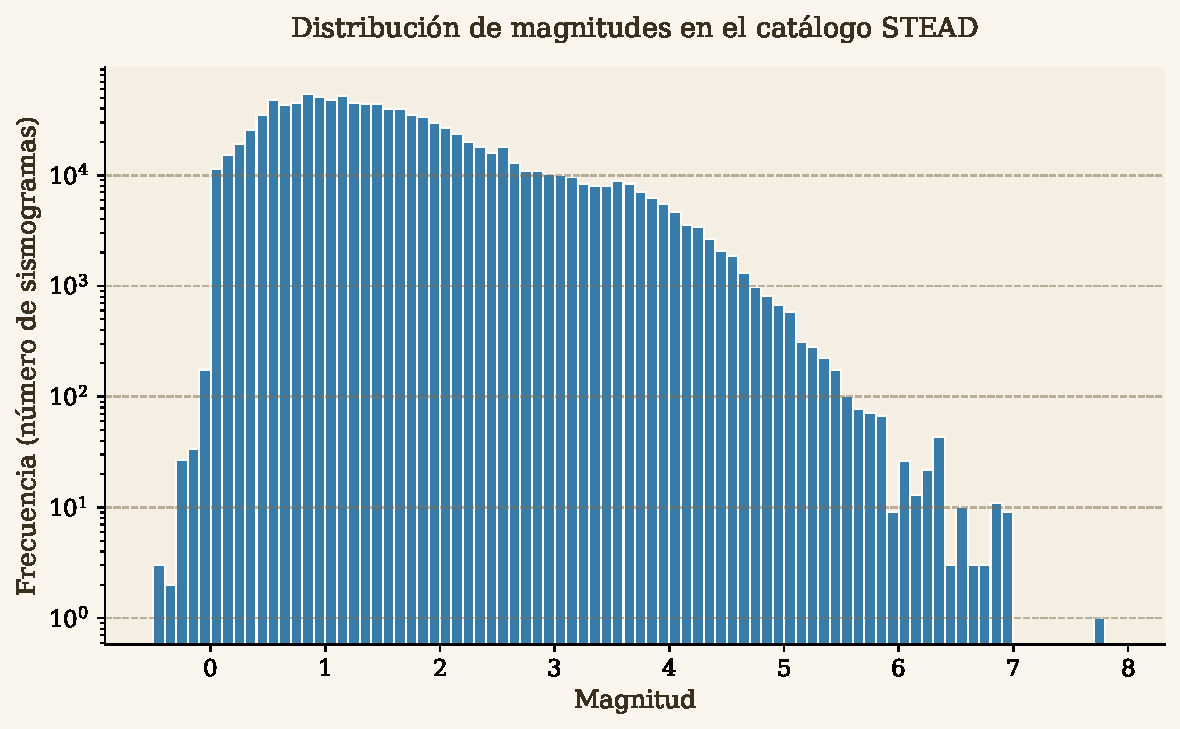
\includegraphics[width=0.85\textwidth]{figuras/figura_histograma_stead}
  \caption[Distribución de magnitudes en el catálogo STEAD]{\textbf{Distribución de magnitudes en el catálogo STEAD.} El histograma muestra la frecuencia de los más de un millón de sismos locales en función de su magnitud (\textbf{nótese la escala logarítmica en el eje Y}). La mayor parte de los eventos registrados se concentran en magnitudes bajas (entre 1 y 3), haciendo visibles también los eventos muy pequeños ($<0.5$) y los escasos grandes terremotos, siguiendo la clásica ley de Gutenberg-Richter.}
  \label{fig:histograma-stead}
\end{figure}

\subsection{Organización del catálogo}
El conjunto de datos se clasifica principalmente en dos tipos de registros:
\begin{itemize}
  \item \textbf{Terremotos locales (\texttt{earthquake\_local}):} Alrededor de $1\,050\,000$ trazas que contienen eventos sísmicos confirmados. En ellas, analistas expertos (o algoritmos de alta fiabilidad) han procedido al picado (\emph{picking}) exacto del instante de llegada de las ondas primarias (P) y secundarias (S).
  \item \textbf{Ruido ambiental (\texttt{noise}):} Unas $450\,000$ trazas correspondientes a periodos de inactividad sísmica. Estas muestras son esenciales como clase negativa para prevenir falsos positivos debidos al ruido generado por la actividad humana o ambiental durante el entrenamiento de modelos de clasificación.
\end{itemize}

\subsection{Los ficheros y sus columnas}
La distribución de STEAD se articula en torno a dos archivos principales, vinculados mediante un identificador único para cada evento:
\begin{enumerate}
  \item Un archivo \texttt{.hdf5} estructurado para almacenar de forma eficiente las matrices multidimensionales correspondientes a las formas de onda crudas.
  \item Un archivo \texttt{.csv} que recoge exhaustivamente los \emph{metadatos}, donde cada fila provee las características analíticas de su sismograma asociado.
\end{enumerate}

Entre los atributos más relevantes incluidos en el archivo tabular, destacan los siguientes:

\begin{itemize}
  \item \textbf{\texttt{trace\_name} y \texttt{trace\_category}:} Constituyen el identificador unívoco del registro y su etiqueta de clase primaria (evento sísmico frente a ruido).
  \item \textbf{\texttt{receiver\_code}, \texttt{receiver\_latitude}, \texttt{receiver\_longitude} y \texttt{receiver\_elevation\_m}:} Proporcionan la identificación y ubicación geoespacial exacta de la estación sismológica receptora.
  \item \textbf{\texttt{source\_magnitude} y \texttt{source\_magnitude\_type}:} Documentan la magnitud del evento y la escala empleada (por ejemplo, magnitud local, $M_L$). Estos campos son exclusivos de los registros clasificados como terremotos.
  \item \textbf{\texttt{source\_latitude}, \texttt{source\_longitude} y \texttt{source\_depth\_km}:} Describen las coordenadas geográficas del epicentro y la profundidad focal de la ruptura (en kilómetros).
  \item \textbf{\texttt{source\_distance\_km} y \texttt{back\_azimuth\_deg}:} Cuantifican la distancia hipocentral y el azimut de propagación, parámetros críticos para caracterizar la atenuación geométrica de las ondas.
  \item \textbf{\texttt{p\_arrival\_sample} y \texttt{s\_arrival\_sample}:} Variables objetivo (\textit{ground truth}) fundamentales para las tareas de regresión temporal; especifican el índice exacto de la muestra discreta ($0$--$5\,999$) correspondiente a los tiempos de llegada de ambas fases.
  \item \textbf{\texttt{p\_status} y \texttt{s\_status}:} Indican la procedencia del picado temporal, distinguiendo entre la intervención de un analista humano (\texttt{manual}) y los sistemas algorítmicos (\texttt{automatic}).
  \item \textbf{\texttt{snr\_db}:} Miden la relación señal-ruido empírica. Valores elevados garantizan una delimitación más nítida de la señal sísmica frente a las perturbaciones de fondo.
\end{itemize}

A partir de este conjunto estructurado, es posible diseñar y entrenar arquitecturas de \textit{Deep Learning} para abordar de manera conjunta la clasificación binaria de la señal (basada en \texttt{trace\_category}) y la regresión precisa de los tiempos de llegada de las fases principales (\texttt{p\_arrival\_sample} y \texttt{s\_arrival\_sample}).

\paragraph{Uso en este TFM.}
En el presente trabajo, se emplean modelos fuertemente consolidados en la literatura, tales como PhaseNet \citep{zhu2018phasenet} y EQTransformer \citep{mousavi2020eqtransformer}, aprovechando su preentrenamiento previo sobre el corpus STEAD mediante la plataforma \emph{SeisBench} \citep{woollam2022seisbench}. Se procede a la validación de sus capacidades predictivas sin requerir un ajuste fino adicional (\textit{zero-shot evaluation}), evaluando su precisión en el picado de fases P y S sobre un subconjunto independiente de eventos y contrastando sus resultados frente a las anotaciones originales del catálogo.

\section{Trabajos relacionados y huecos identificados}
\label{trabajos-relacionados}

La revisión bibliográfica realizada permite identificar el posicionamiento específico de este TFM frente al estado del arte:

\begin{itemize}
  \item \textbf{Frente a ETAS}: el enfoque propuesto retiene la formalización probabilística pero sustituye la forma funcional fija por arquitecturas DL que pueden descubrir patrones no contemplados a priori \citep{ogata1998spacetime, vandenende2024forecasting}.

  \item \textbf{Frente a UCERF3}: UCERF3-ETAS \citep{field2017ucerf3etas} es un modelo operacional consolidado, mientras que el sistema aquí\, propuesto es un prototipo de investigación. No se busca por tanto competir directamente en escala operativa, sino mostrar \emph{si} el DL aporta ganancia metrológicamente significativa sobre los \textit{baselines} clásicos en una región bien caracterizada (California).

  \item \textbf{Frente a PhaseNet/EQTransformer}: estos modelos resuelven el problema \emph{previo} al pronóstico (detección y \textit{picking}). En este TFM se reutilizan como \emph{front-end} preentrenado para alimentar el \emph{back-end} de pronóstico, sin re-entrenarlos.

  \item \textbf{Frente a DeVries et al. (2018) y Rouet-Leduc et al. (2017)}: los trabajos previos más cercanos abordan, respectivamente, la predicción espacial de réplicas y la predicción temporal en laboratorio. Este TFM combina ambas dimensiones (espacial y temporal) sobre catálogos reales con \emph{declustering} explícito para aislar mainshocks independientes.

  \item \textbf{Hueco principal:} la mayoría de los trabajos recientes evaluan un único modelo contra \textit{baselines} débiles, con una sola semilla o sin tests estadísticos. Este TFM aplica en su metodología una comparación exhaustiva y rigurosa \citep{beroza2021dlreview, reichstein2019deep}: multi-semilla, Wilcoxon pareado, multiples \textit{baselines} interpretables, y reproducibilidad estricta.
\end{itemize}

\section{Síntesis}
\label{sintesis}

Las bases teóricas y empíricas revisadas permiten formular tres hipótesis operativas que guiarán la fase experimental:

\begin{enumerate}[label=\textbf{H\arabic*.}]
  \item Las redes preentrenadas \emph{PhaseNet} y \emph{EQTransformer} permiten ejecutar la detección y \textit{picking} de fases P/S sobre STEAD con calidad comparable a la literatura, sin re-entrenamiento.
  \item Una TCN sobre \textit{features} globales del catálogo USGS \emph{no} basta para superar a una regresión logística simple sobre las mismas agregaciones; la señal precursora explotable en estas \textit{features} es de naturaleza estadística, no temporal-secuencial.
  \item La incorporación explícita de la dimensión espacial mediante una GNN sobre celdas activas sí\, mejora significativamente sobre los \textit{baselines}, evidenciando que el cuello de botella del pronóstico sísmico con DL no es la complejidad temporal sino la representación espacial.
\end{enumerate}
